% !TeX program = xelatex
\documentclass[12pt, a4paper]{article}
\usepackage{xltxtra}

% ! Language and fonts !
\usepackage{polyglossia}
% language
\setmainlanguage{russian}
\setotherlanguage{english}
% fonts
\setmainfont[Ligatures=TeX]{CMU Serif}
\setromanfont[Ligatures=TeX]{CMU Serif} 
\setsansfont[Ligatures=TeX]{CMU Serif} 
\setmonofont[Ligatures=TeX]{CMU Serif} 
% set fonts to cyrillic
\newfontfamily{\cyrillicfont}[Ligatures=TeX]{CMU Serif}
\newfontfamily{\cyrillicfontrm}[Ligatures=TeX]{CMU Serif}
\newfontfamily{\cyrillicfonttt}[Ligatures=TeX]{CMU Serif} 
\newfontfamily{\cyrillicfontsf}[Ligatures=TeX]{CMU Serif} 
% rename pictures and tables
\addto\captionsrussian{
  \renewcommand{\figurename}{Рис.}
  \renewcommand{\tablename}{Табл.}
}
% math
\usepackage{unicode-math}
\setmathfont{TeX Gyre Termes Math}

% ! Document format !
\usepackage{comment}
\begin{comment}]
\usepackage{geometry} % Задаём поля:
\geometry{left=3cm} % левое — 3 см;
\geometry{right= 1.5cm} % правое — 1,5 см;
\geometry{top=2cm} % верхнее — 2 см;
\geometry{bottom=2cm} % нижнее — 2 см;
\usepackage{setspace} \onehalfspacing % Задаём «полуторный» межстрочный интервал.
\usepackage{indentfirst} % Автоматически добавляем отступ в каждый новый абзац.
\usepackage[all]{nowidow} % Пакет для борьбы с «висячими» строками абзацев, лучшая альтернатива переопределению \clubpenalty и \widowpenalty.
\usepackage{enumitem} % Настраиваем работу со списками:
\def\labelitemi{—} % задаём длинное тире как стандартный маркер ненумерованного списка;
\setlist{nolistsep} % убираем дополнительные отступы между элементами списка;
\usepackage{fancyhdr} % Настраиваем колонтитулы:
\pagestyle{fancy} % задаём макет страницы, отличный от стандартного;
\fancyhf{} % сбрасываем содержимое колонтитулов;
\renewcommand{\headrulewidth}{0pt} \renewcommand{\footrulewidth}{0pt} % убираем декоративные линии из колонтитулов;
\fancyfoot[C]{\thepage} % настраиваем расположение номера страницы в нижнем колонтитуле: L — слева, R — справа, C — по центру.
\addto\captionsenglish{\renewcommand{\partname}{}} % меняем имя главы
\setcounter{part}{-\maxdimen} % убираем счет глав
\usepackage{titlesec} % настраиваем заголовки частей документа:
\titleformat*{\section}{\newpage\normalsize\bfseries\centering} % настраиваем заголовок раздела; начинаем каждый раздел с новой страницы; размер шрифта — такой же, как во всем документе, начертание — полужирное, выравнивание  — по центру.
\end{comment}

% ! useful package !
\setlength{\mathsurround}{2pt}
\usepackage{mathtext}
\usepackage{booktabs,tabulary,tabularx,longtable}
\newcolumntype{M}[1]{>{\centering\arraybackslash}m{#1}} % resize row
\newcolumntype{N}{@{}m{0pt}@{}} % zero row
\usepackage{array} % for extrarowheight
\usepackage{varwidth} % for the varwidth minipage environment
\usepackage{graphicx} 
\usepackage{listings} 
\usepackage{color} 
\usepackage{xunicode}
\usepackage{ulem}

\usepackage{sectsty}

\allsectionsfont{\centering}
\setcounter{secnumdepth}{0}

\usepackage{multicol}
\usepackage{lipsum}
\usepackage{mwe}
\usepackage{float}

\usepackage[left=2cm,right=2cm,top=2cm,bottom=2.5cm]{geometry}

\author{Круглов Иван, Кузнецов Илья} 
\title{\textbf{Обзор Intellij IDEA}} 
\date{\today} 

\addto\captionsrussian{
  \renewcommand{\contentsname}
    {Мы будем исследовать такие функции как}
}
\begin{document}

    % page 1
    \begin{Huge}
        \maketitle
    \end{Huge}

    % page 2
    \newpage
    \tableofcontents

    
    % page 3
    \newpage
    \section{Создание проекта}
    При открытие IDE мы попадаем на стартовое окно создания/загрузки проекта
    
    \begin{figure}[H]
        \centering{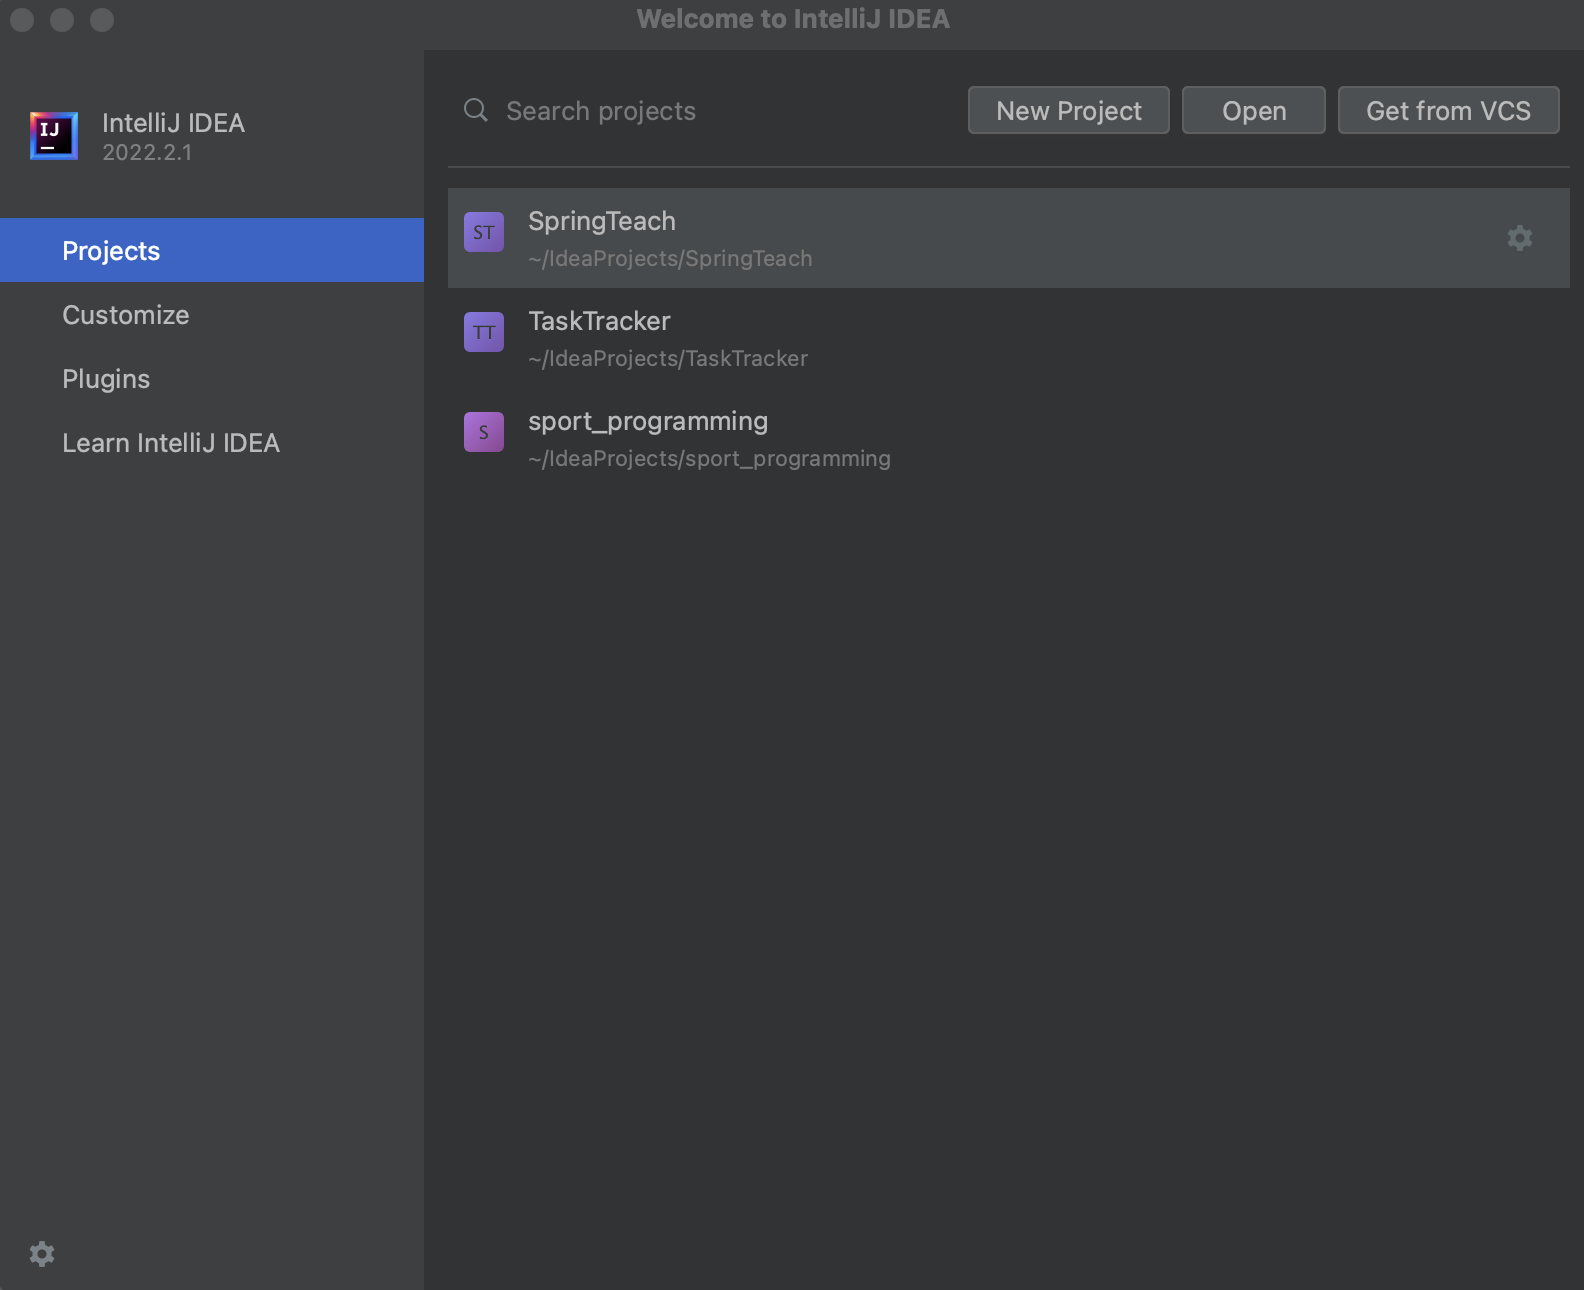
\includegraphics[width=0.8\linewidth]{src/start.png}}
        \caption{Выбор дальнейшего действия}
    \end{figure}

    Далее мы можем сделать выбор, что мы хотим сделать с проектом:
    \begin{itemize}
        \item Создать новый
        \item Открыть существующий
        \item Или же скопировать проект из системы контроля версий (git, github, gitlab, etc.)
    \end{itemize}
    

    % page4
    \newpage
    \subsection{Создаем новый проект}

    Производим первоначальную настройку нашего проекта:
    
    \begin{figure}[H]
        \centering{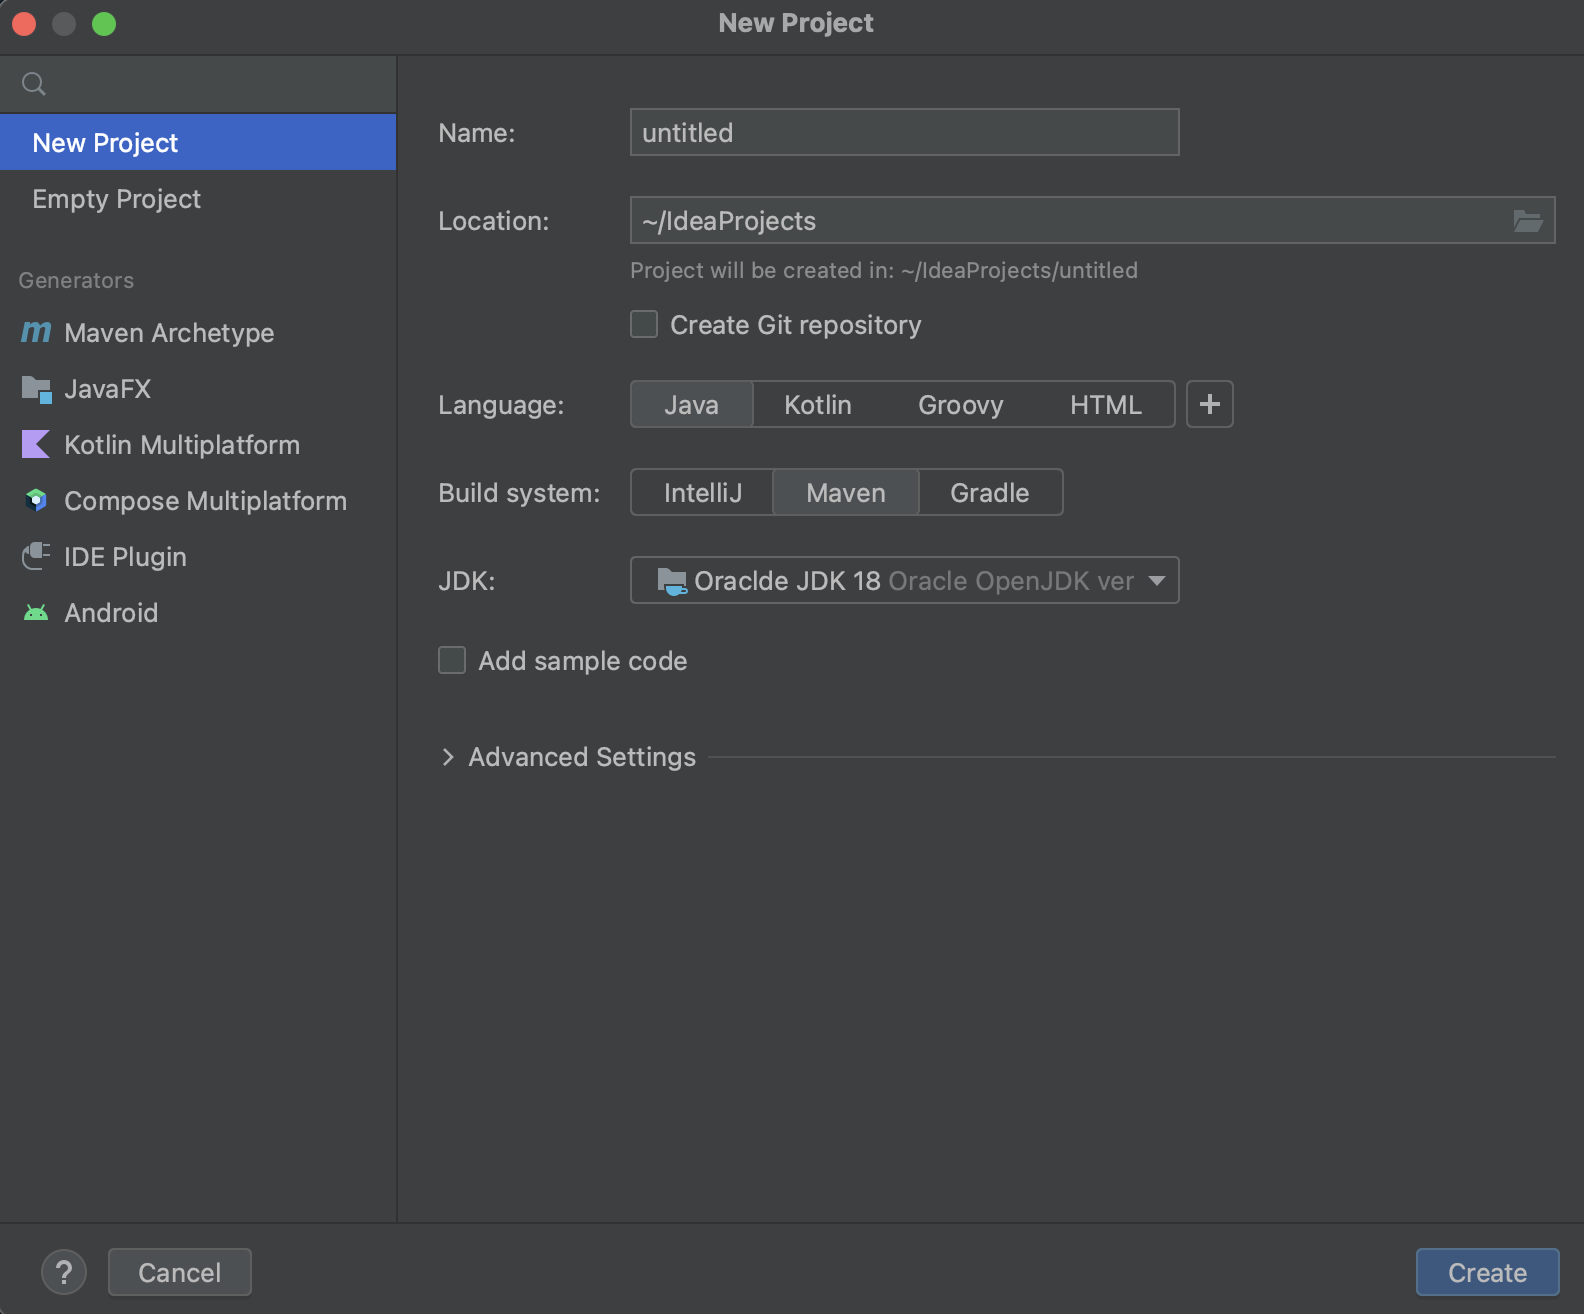
\includegraphics[width=0.8\linewidth]{src/newproj.png}}
        \caption{Создание проекта}
    \end{figure}

    Обычно для настройки нам достаточно
    \begin{itemize}
        \item Ввести название проекта
        \item Выбрать ЯП (для нас это будет java)
        \item Выбрать систему сборки (Рассмотрим в случае с Maven)
        \item Создать или не создавать локальный репозиторий для проекта
        \item Выбрать доступную JDK\\
        Если таковых не существует, в том же окне нам предложат авоматически установить новую
    \end{itemize}


    % page 5
    \newpage
    \subsection{Копируем проект из VCS}
    
    \begin{figure}[H]
        \centering{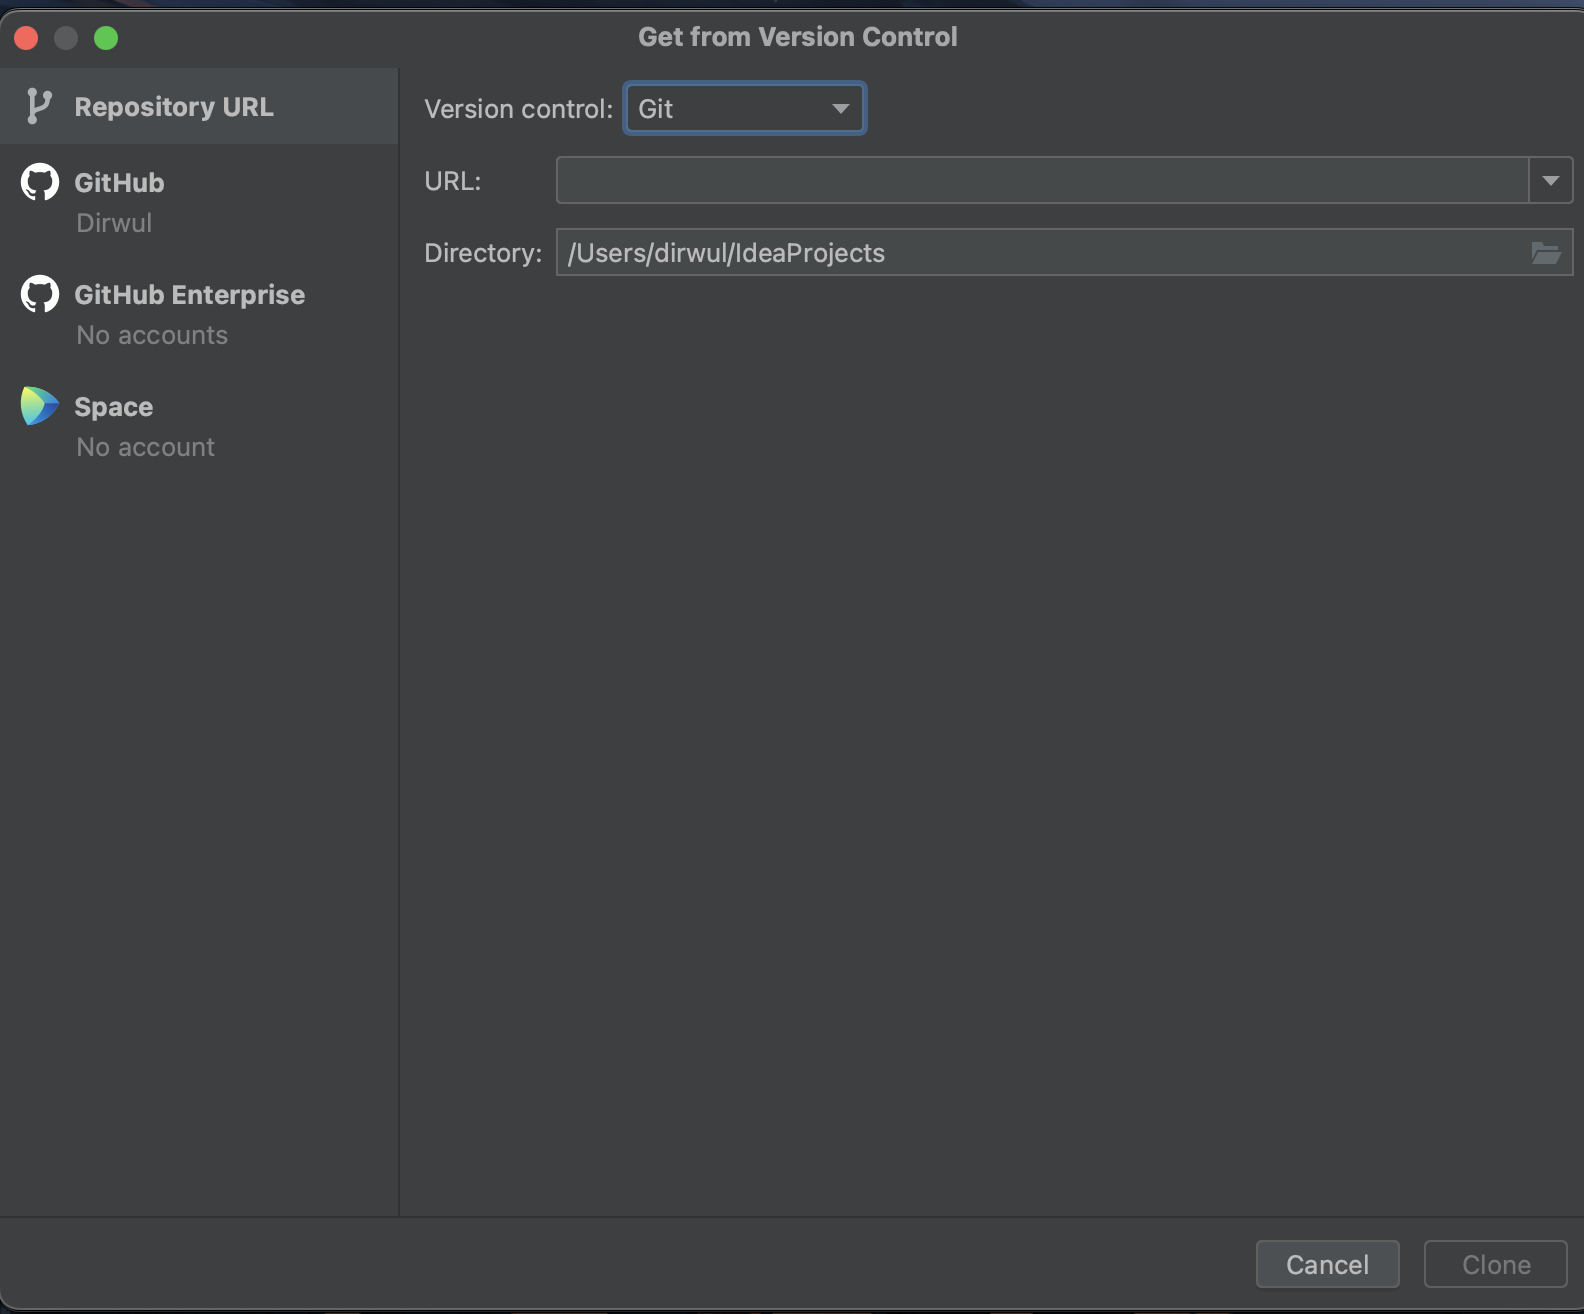
\includegraphics[width=0.8\linewidth]{src/getfromvcs.png}}
        \caption{Выбор VCS}
    \end{figure}

    В данном окне нам предоставляется выбор:

    \begin{itemize}
        \item Скопировать репозиторий по URL
        \item Залогиниться в GitHub и выбрать репозиторий оттуда
        \item Выбрать репозиторий из GitHub Enterprise
        \item Выбрать репозиторий из JetBrains Space
    \end{itemize}

    % page 6
    \newpage
    \section{Создание первой программы на Java}

    \subsection{Создание java class'a}

    Для создания первой программы на Java нам потребуется спуститься по папкам: src -> main -> java 
    и создать там наш первый Java-class.

    \begin{figure}[H]
        \centering{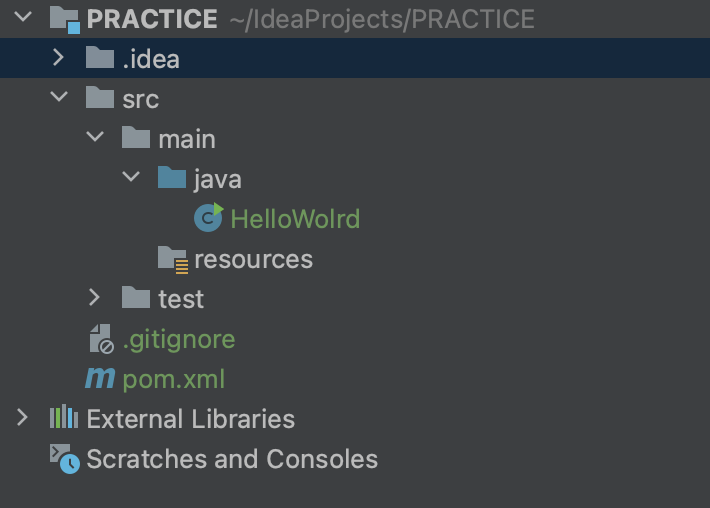
\includegraphics[width=0.4\linewidth]{src/tree.png}}
        \caption{Правильная директория для класса в Maven}
    \end{figure}

    Так же при создании класса IDE предложит добавить наш файл в git(отслеживать его)

    \begin{figure}[H]
        \centering{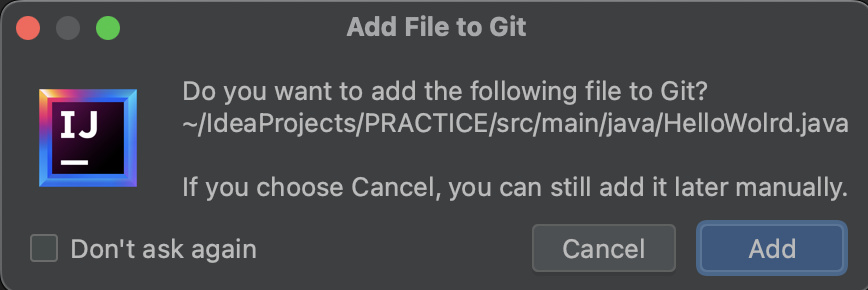
\includegraphics[width=0.4\linewidth]{src/addfiletogit.png}}
        \caption{Добавление в git}
    \end{figure}

    Исходный код нашего Hello world выглядит так:
    
    \begin{figure}[H]
        \centering{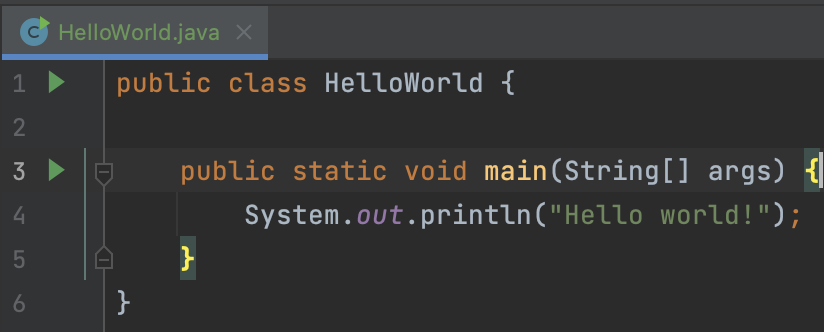
\includegraphics[width=0.75\linewidth]{src/hello.png}}
        \caption{Hello wolrd}
    \end{figure}

    \subsection{Создание конфигурации для запуска}

    Чтобы запустить наш java class нам потребуется создать конфигурацию и настроить ее:

    \begin{figure}[H]
        \centering{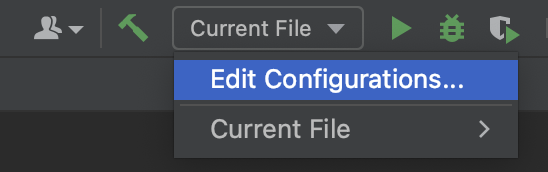
\includegraphics[width=0.4\linewidth]{src/startconf.png}}
        \caption{Заходим в настройки конфигурации}
    \end{figure}

    В настройках конфигурации нас интересует два параметра:
    \begin{itemize}
        \item Название конфигурации, которое ни на что не влияет, но в реальном проекте у нас может быть
        несколько конфигураций запуска
        \item Main класс для запуска (HelloWorld)
    \end{itemize}

    
    \begin{multicols}{2}[]
        \begin{figure}[H]
            \centering{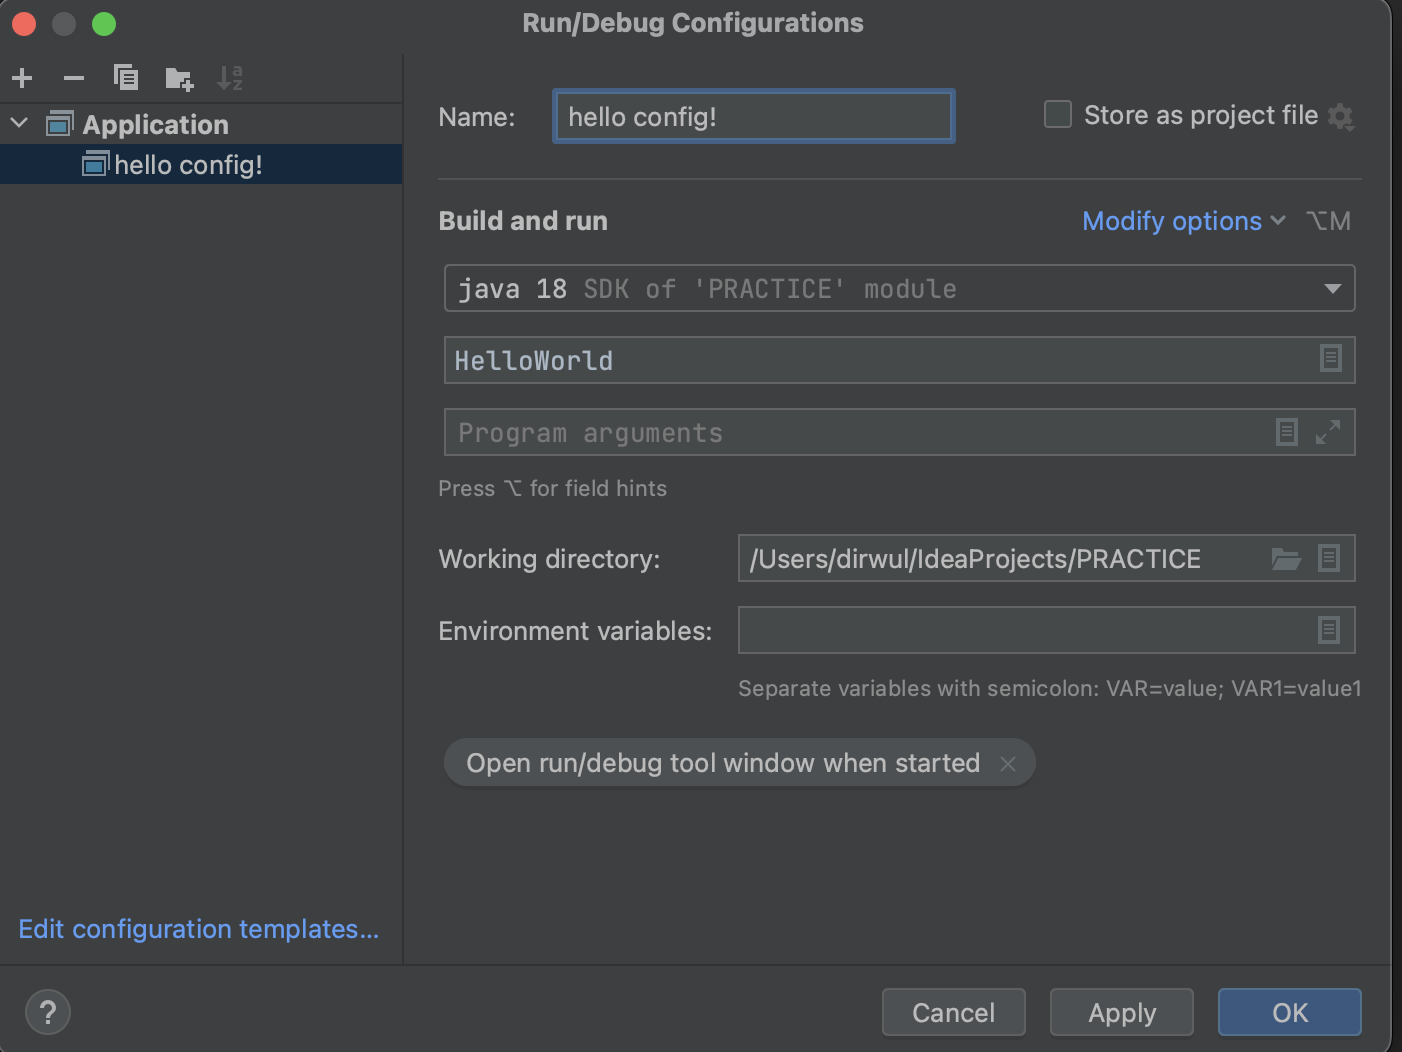
\includegraphics[width=\linewidth]{src/createconfig.png}}
            \caption{Создаем конфигурацию}
        \end{figure}
        \columnbreak
        \begin{figure}[H]
            \centering{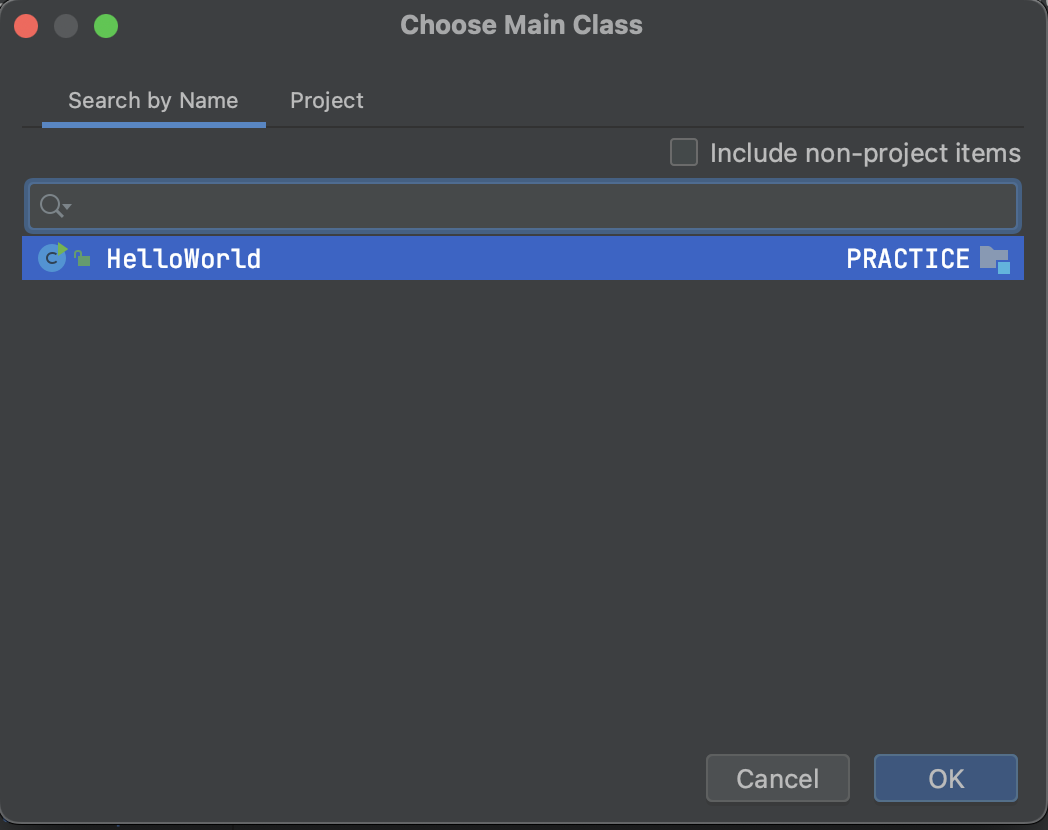
\includegraphics[width=\linewidth]{src/choosemainclass.png}}
            \caption{Окно выбора main-class'a}
        \end{figure}
    \end{multicols}

    \begin{comment}
    \begin{figure}[H]
        \centering{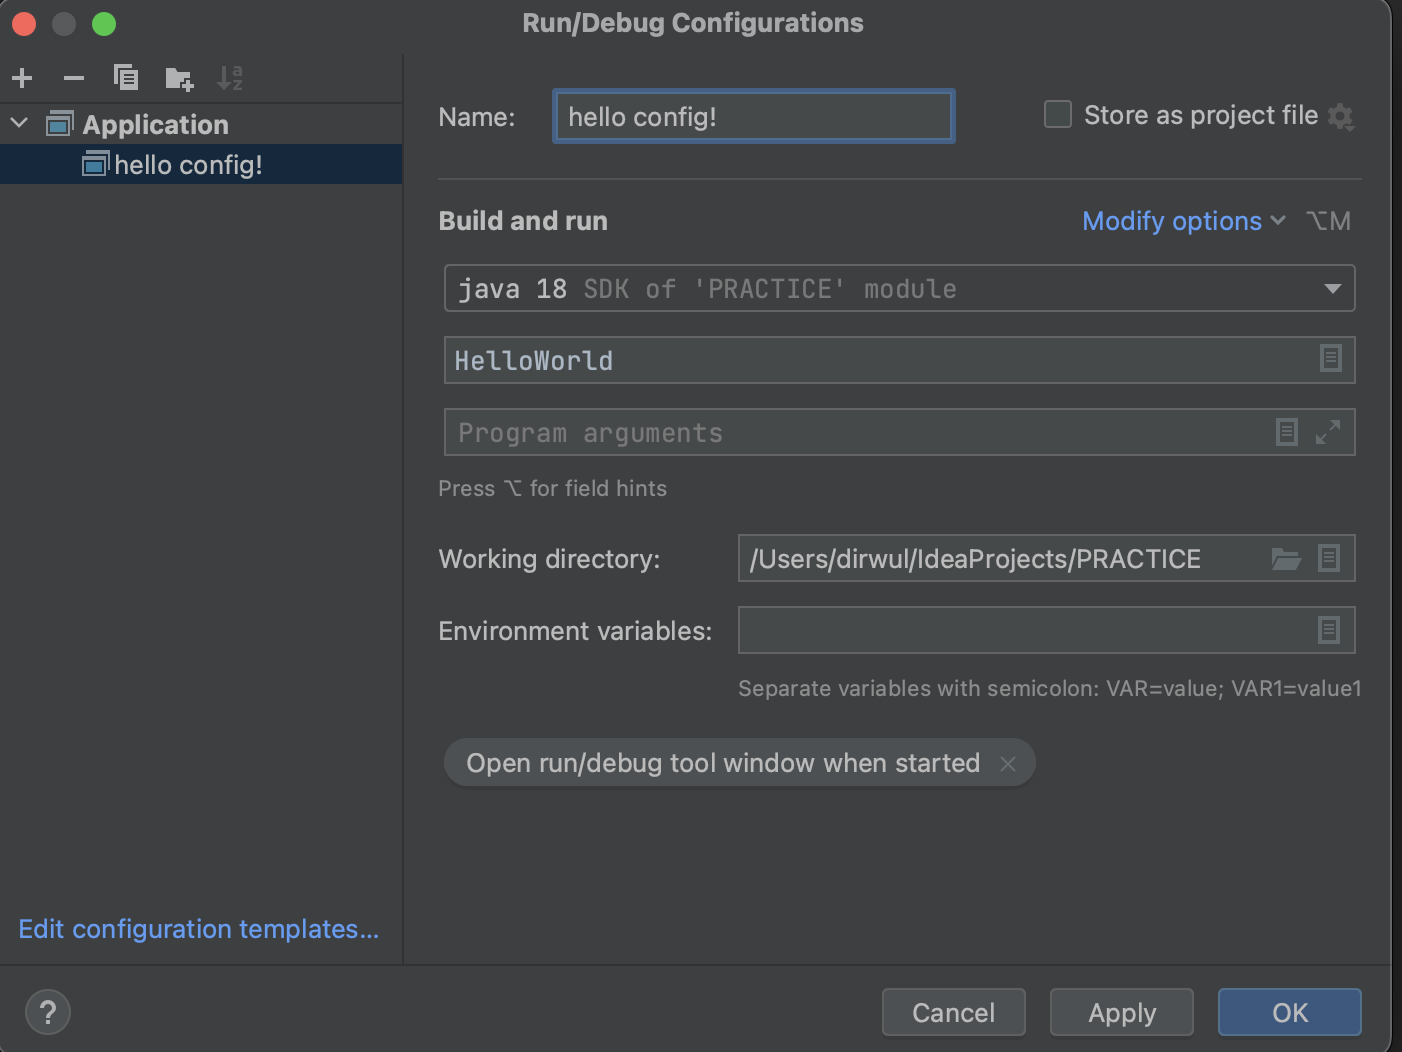
\includegraphics[width=0.75\linewidth]{src/createconfig.png}}
        \caption{Создаем конфигурацию}
    \end{figure}

    \begin{figure}[H]
        \centering{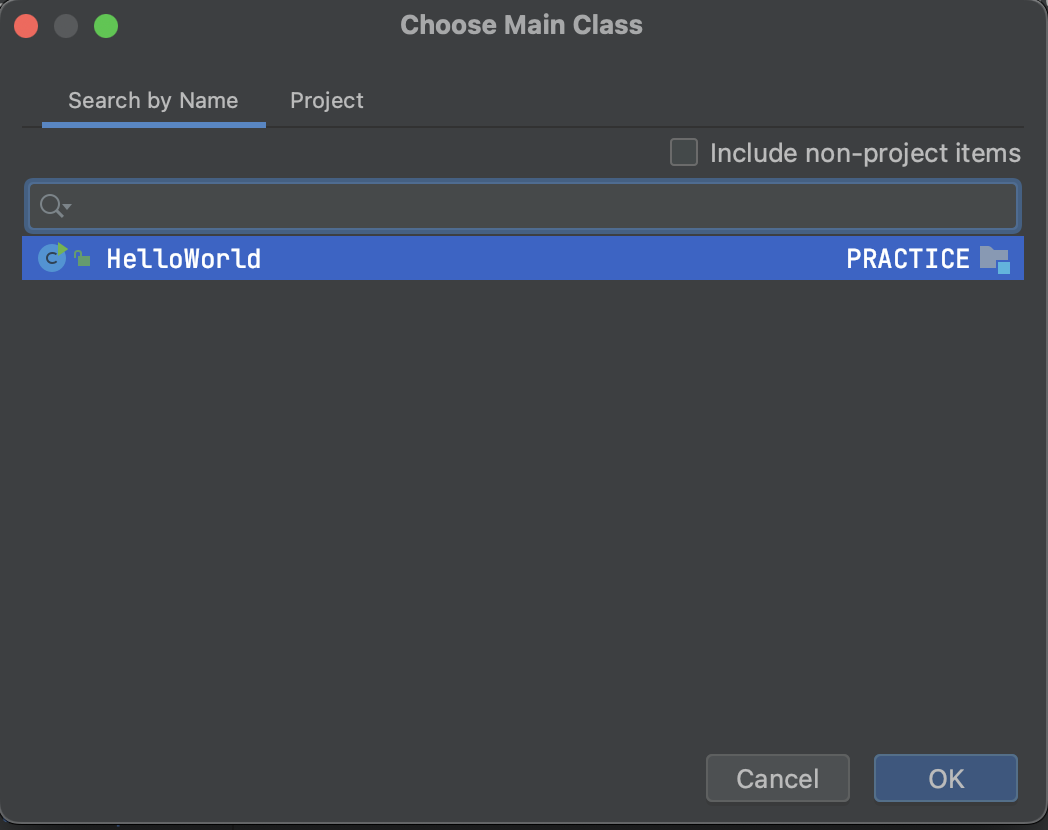
\includegraphics[width=0.75\linewidth]{src/choosemainclass.png}}
        \caption{Окно выбора main-class'a}
    \end{figure}
\end{comment}

    % page 7
    \newpage
    \section{Запуск и отладка}

    \subsection{Стандартный запуск}
    
    \textit{Здесь и далее, все использованные хоткеи будут озвучиваться для MacOS,
    однако на windows в бОльшинстве слуаев достаточно заменить системные клавиши на эквивалетные}\\
    
    Для запуска программы нам достаточно нажать \textit{ctrl+R} и созданная нами ранее конфигурация запустит наш Java class.
    После чего снизу откроется окно консоли с выводом программы на экран:

    \begin{figure}[H]
        \centering{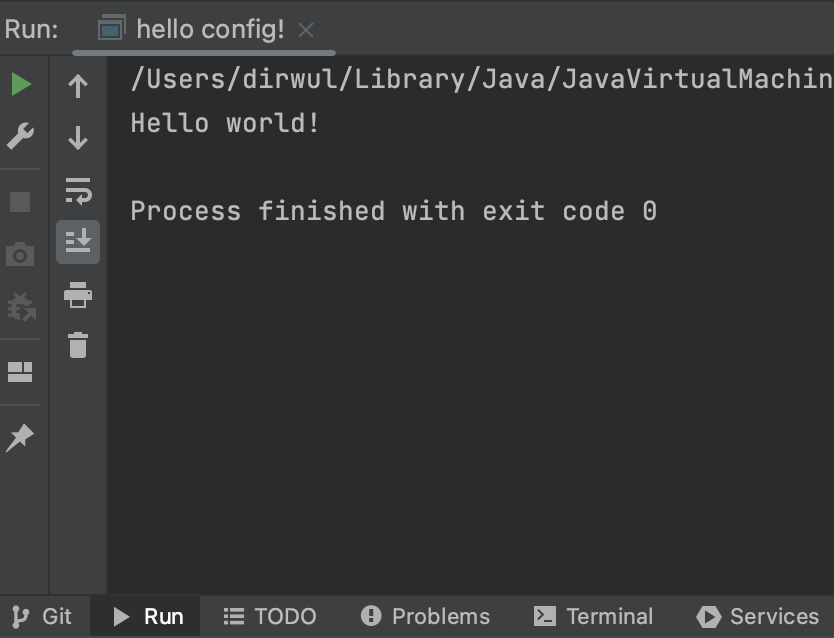
\includegraphics[width=0.5\linewidth]{src/output.png}}
        \caption{Output window}
    \end{figure}

    \subsection{Запуск в режиме отладки}

    Теперь немного усложним программу, добавим в нее две переменные и вывод на экран "Hello break point".
    Вывод этой строки на экран отметим как breakpoint.
    
    \begin{figure}[H]
        \centering{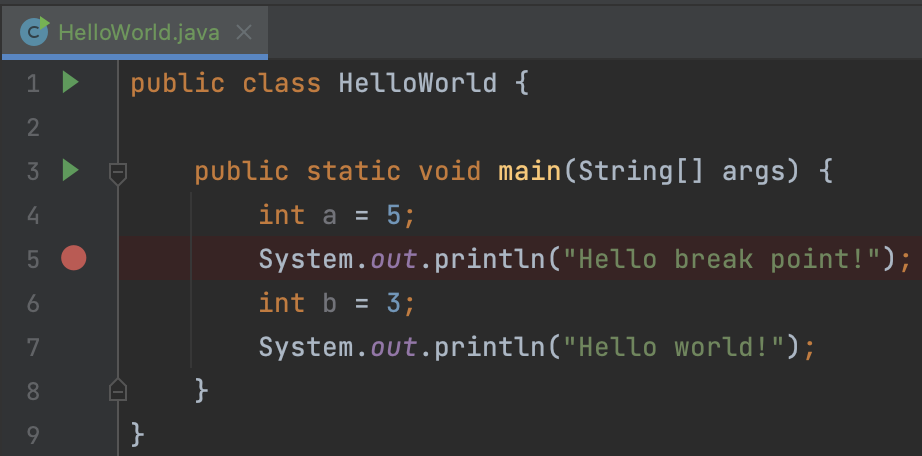
\includegraphics[width=0.75\linewidth]{src/breakpoint.png}}
        \caption{Создание breakpoint'a}
    \end{figure}

    Теперь запустим нашу программу в режиме отладки \textit{(ctrl+D)}
    
    \begin{figure}[H]
        \centering
        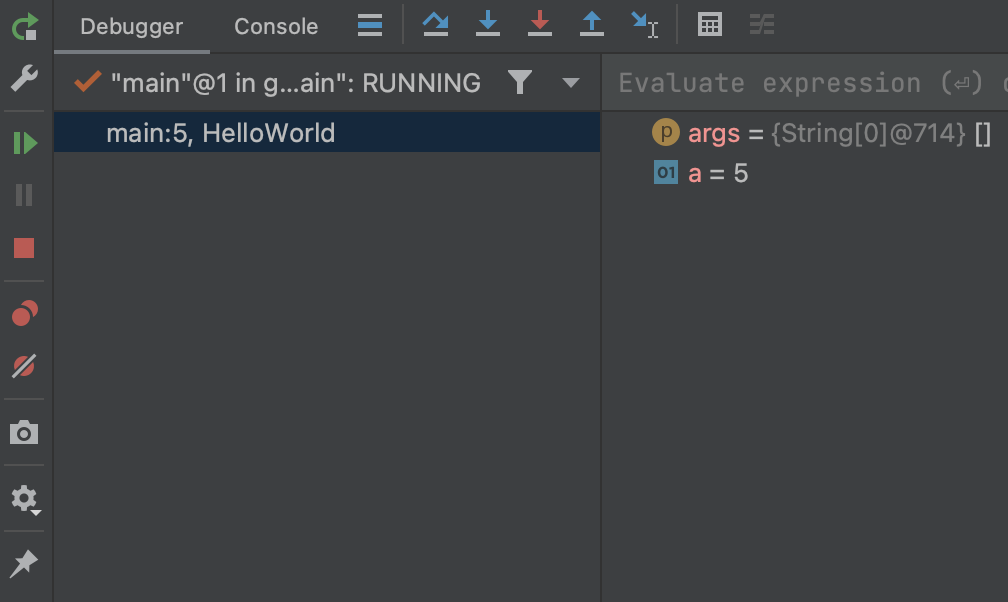
\includegraphics[width=0.75\linewidth]{src/output2.png}
        \caption{Состояние переменных на момент остановки у breakpoint'a}
    \end{figure}

    То есть в режиме отладки IDE позволяем нам перемещаться от одного breakpoint'a к другому, 
    зная состояние каждой переменной на каждом шагу, что, несомненно, очень удобно при отладке 
    приложений.


    % page 8
    \newpage
    \section{Настройки и форматирование}

    Общие настройки проекта, форматирования и т.д. доступны при нажатии на \textit{command + ,}
    Рассматривать их не имеет смысла в данном случае, т.к. их слишком много и каждый подбирает настройки под себя
    Поэтому пройдемся по основным пунктам:
    \begin{itemize}
        \item Общие настройки IDE
        \item Хоткеи
        \item Редактор кода
        \item VCS и все с ними связанное
        \item Настройки билда, компилятора и дебаггера
        \item Находящиеся под управлением IDE языки и фреймворки
        \item Прочие инструменты
        \item Расширенные настройки
    \end{itemize}

    \begin{figure}[H]
        \centering
        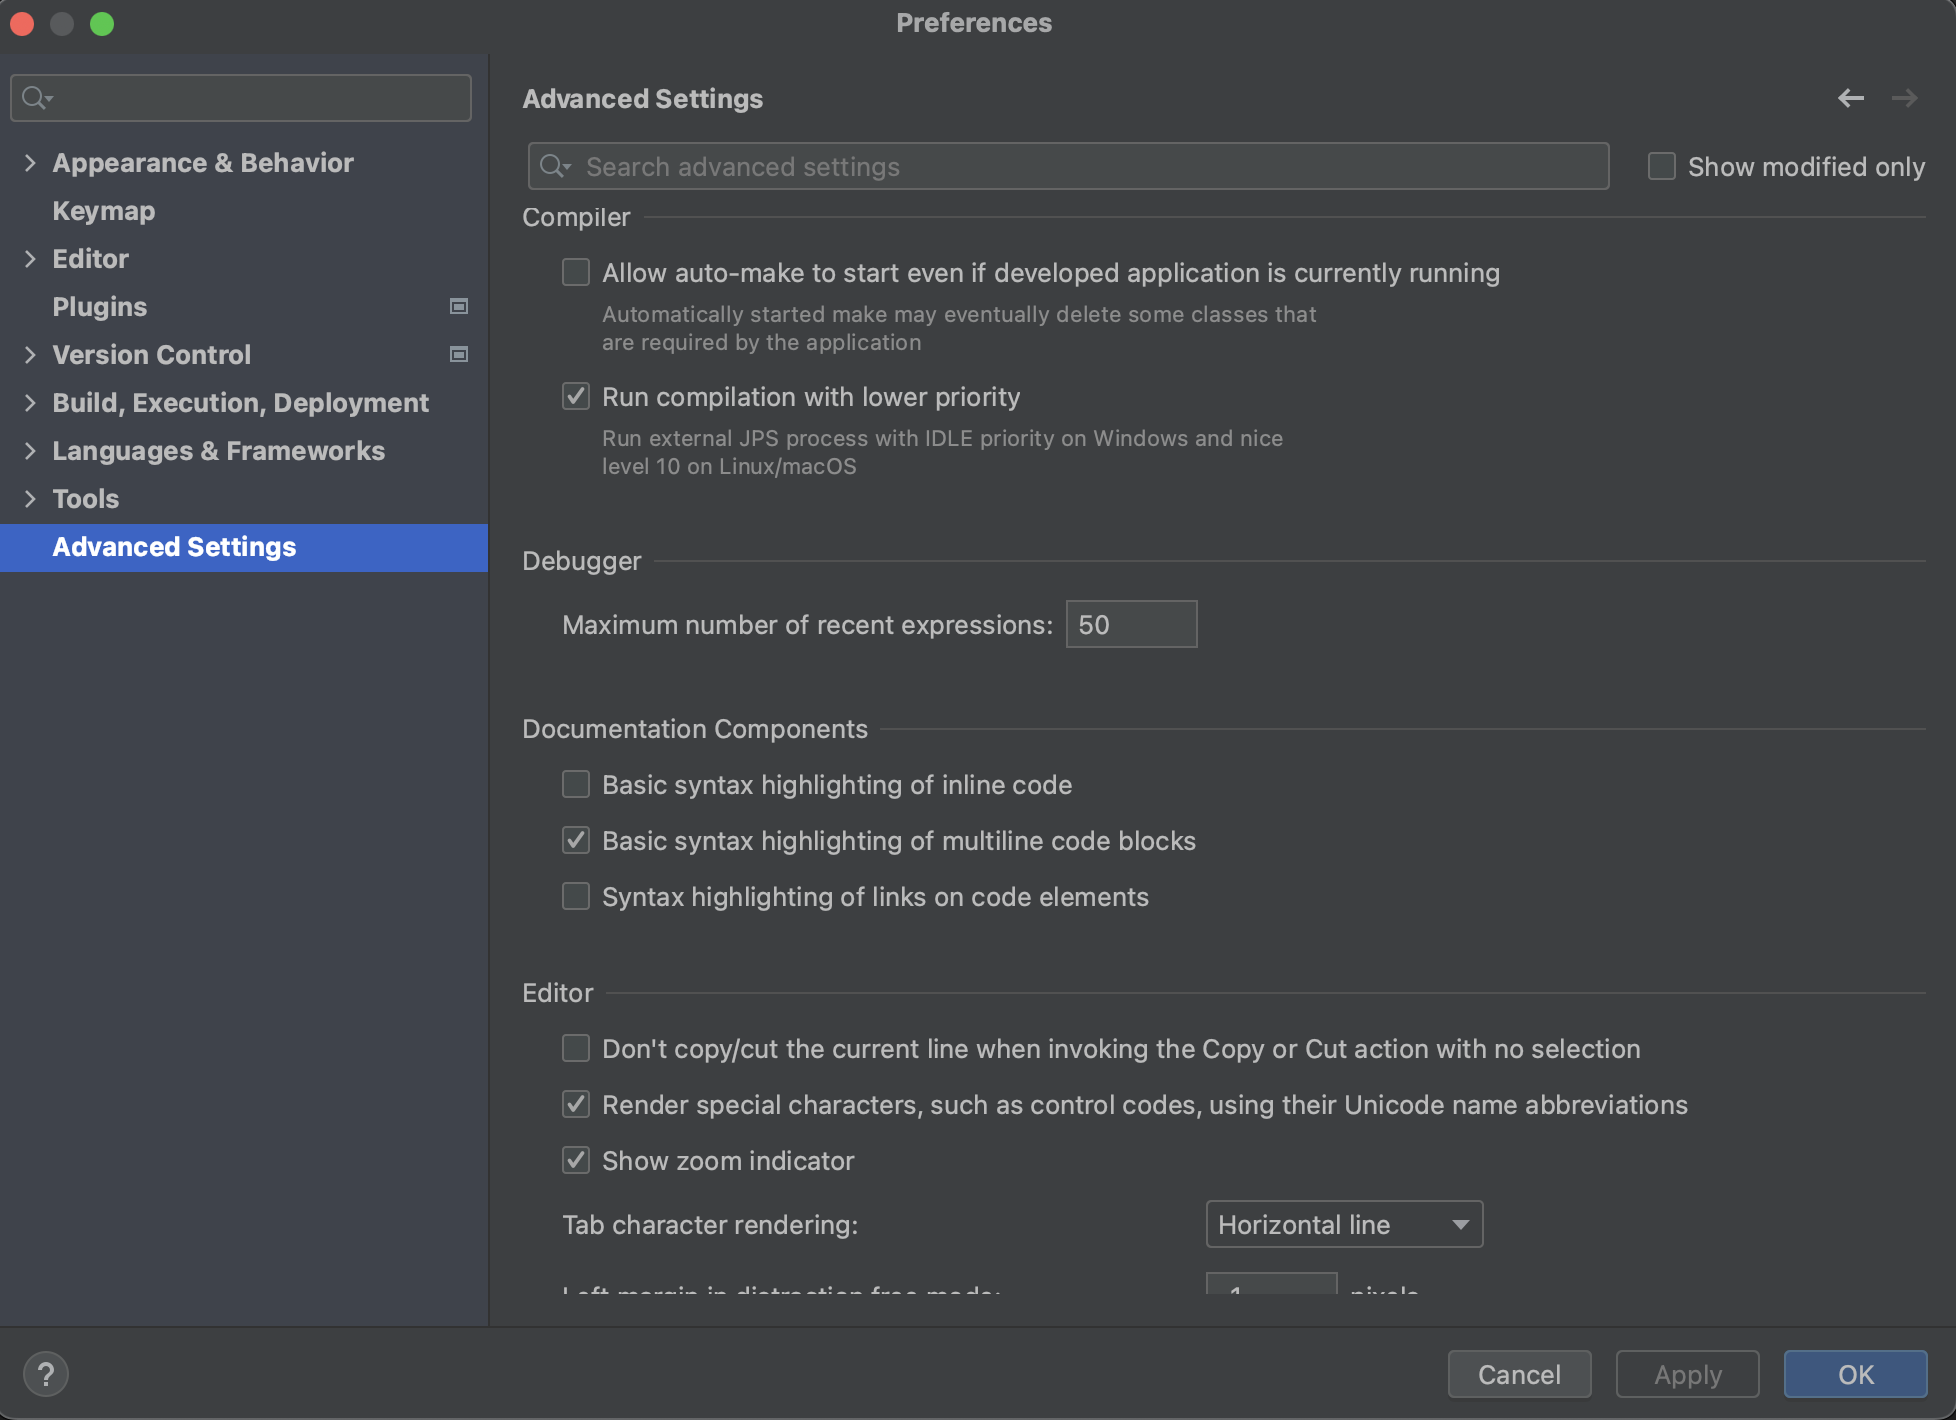
\includegraphics[width=0.75\linewidth]{src/preferences.png}
        \caption{Настройки}
    \end{figure}

    Форматирование кода для всего файла можно запустить через \textit{option + command + L}

    \begin{figure}[H]
        \centering
        
\includegraphics[width=0.75\linewidth]{src/format.png}
        \caption{Форматирование}
    \end{figure}
    

    % page 9
    \newpage
    \section{Настройка репозитория}
    
    Чтобы создать удаленный репозиторий, нам достатоточно запушить что-либо в него.
    Предварительно так же требуется залогиниться в github/gitlab/other vcs.
    Рассмотрим пример с гитхабом, где нам доступно две опции:
    
    \begin{itemize}
        \item Редирект ссылка на github
        \item Создание специального токена
    \end{itemize}

    \begin{figure}[H]
        \centering
        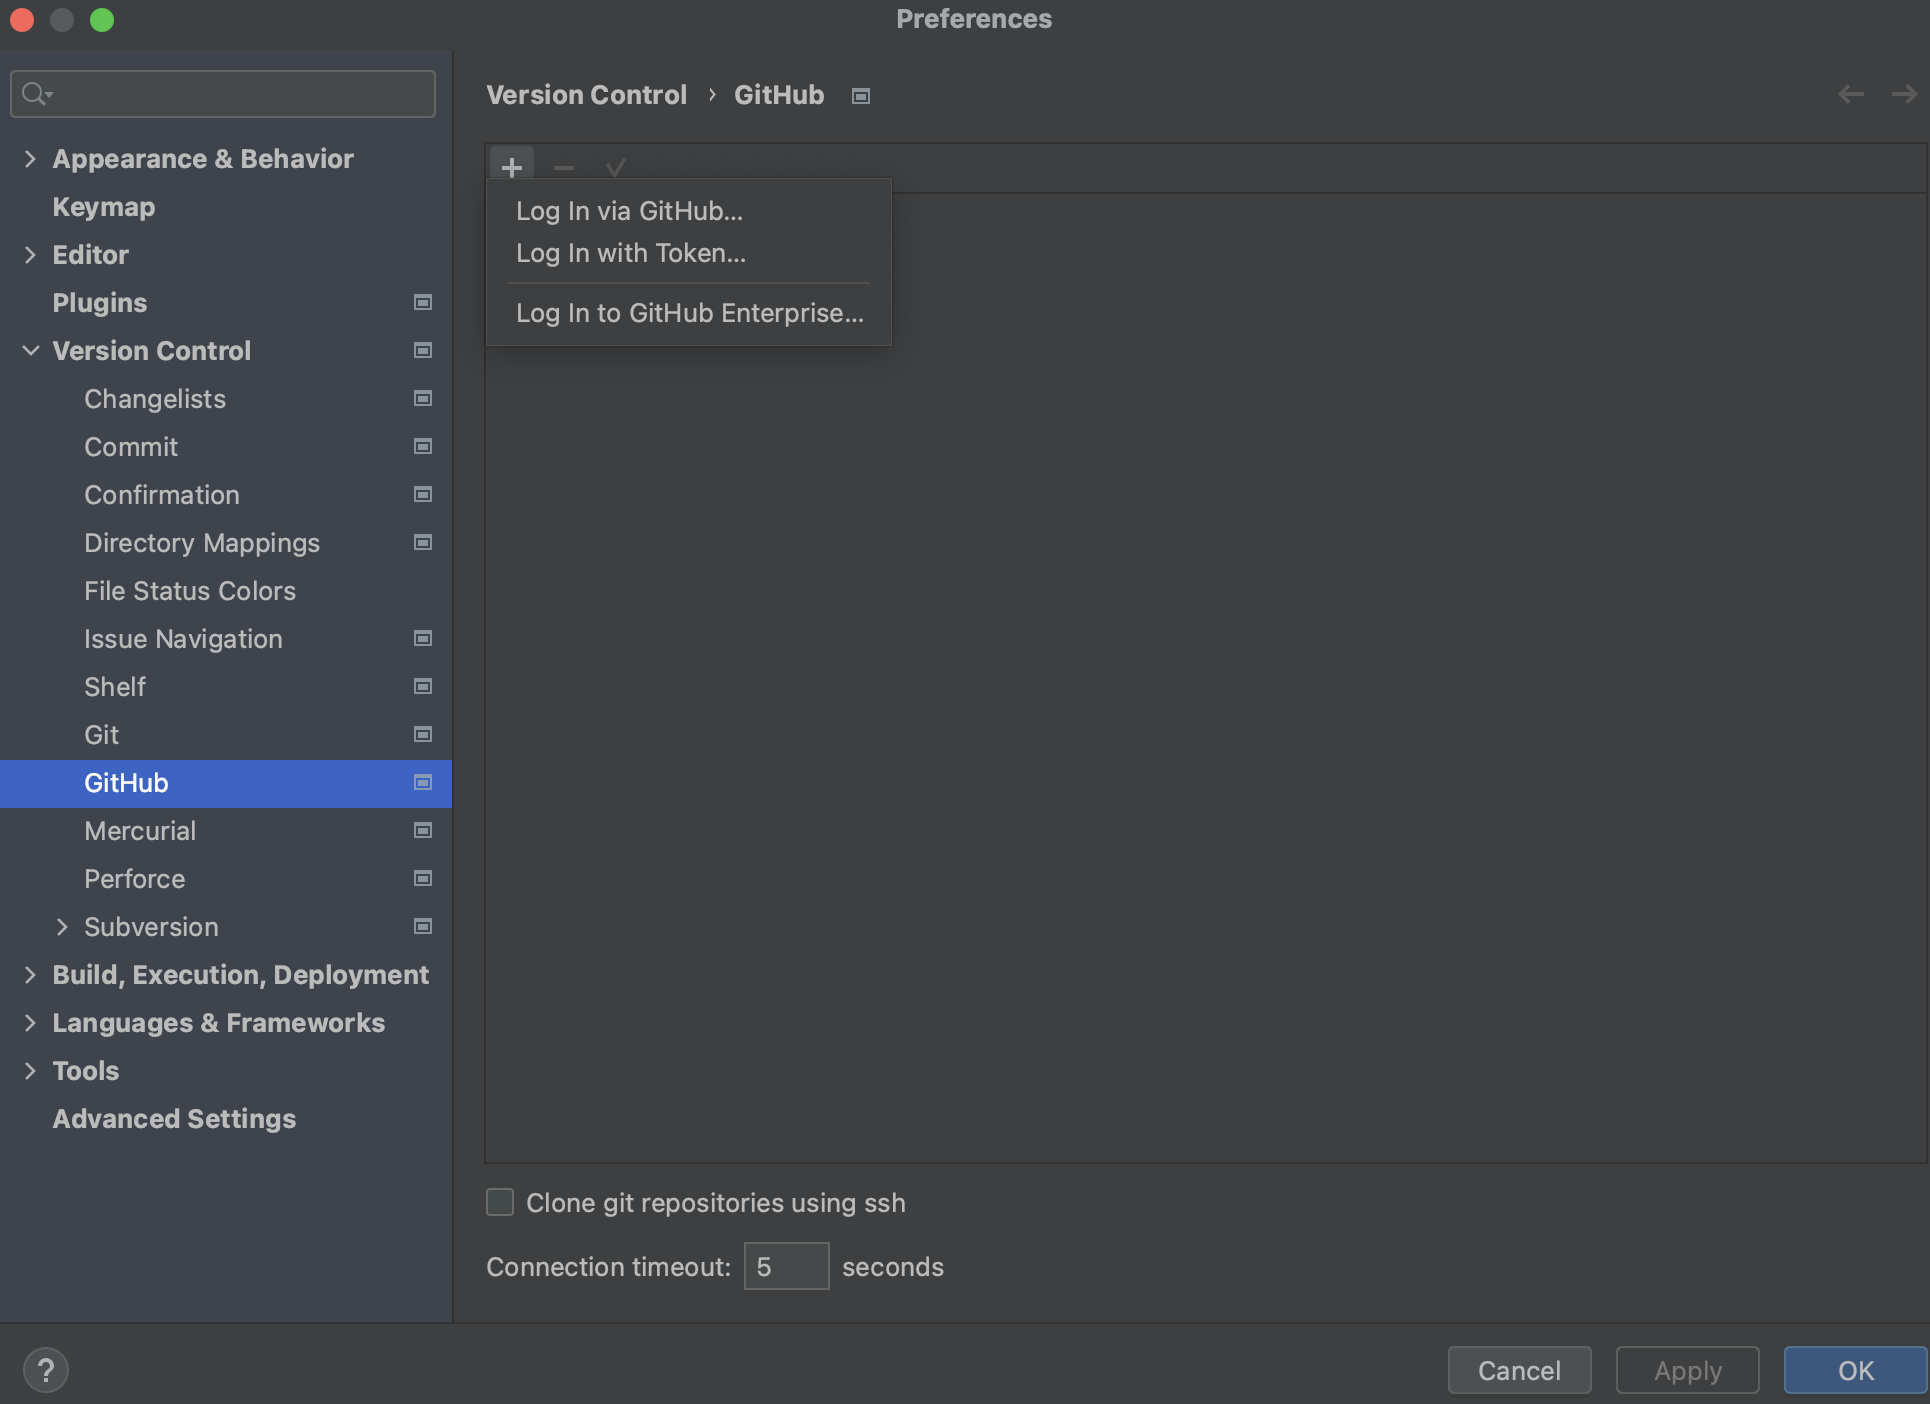
\includegraphics[width=0.75\linewidth]{src/login.png}
        \caption{Логин в гитхаб}
    \end{figure}

    Также нам требуется обновить .gitignore
    Сделаем папку \textit{.idea} и файл \textit{pom.xml} 
    нетрекаемыми \textit{(я не знаю как правильно это называется)} для git
    
    \begin{figure}[H]
        \centering
        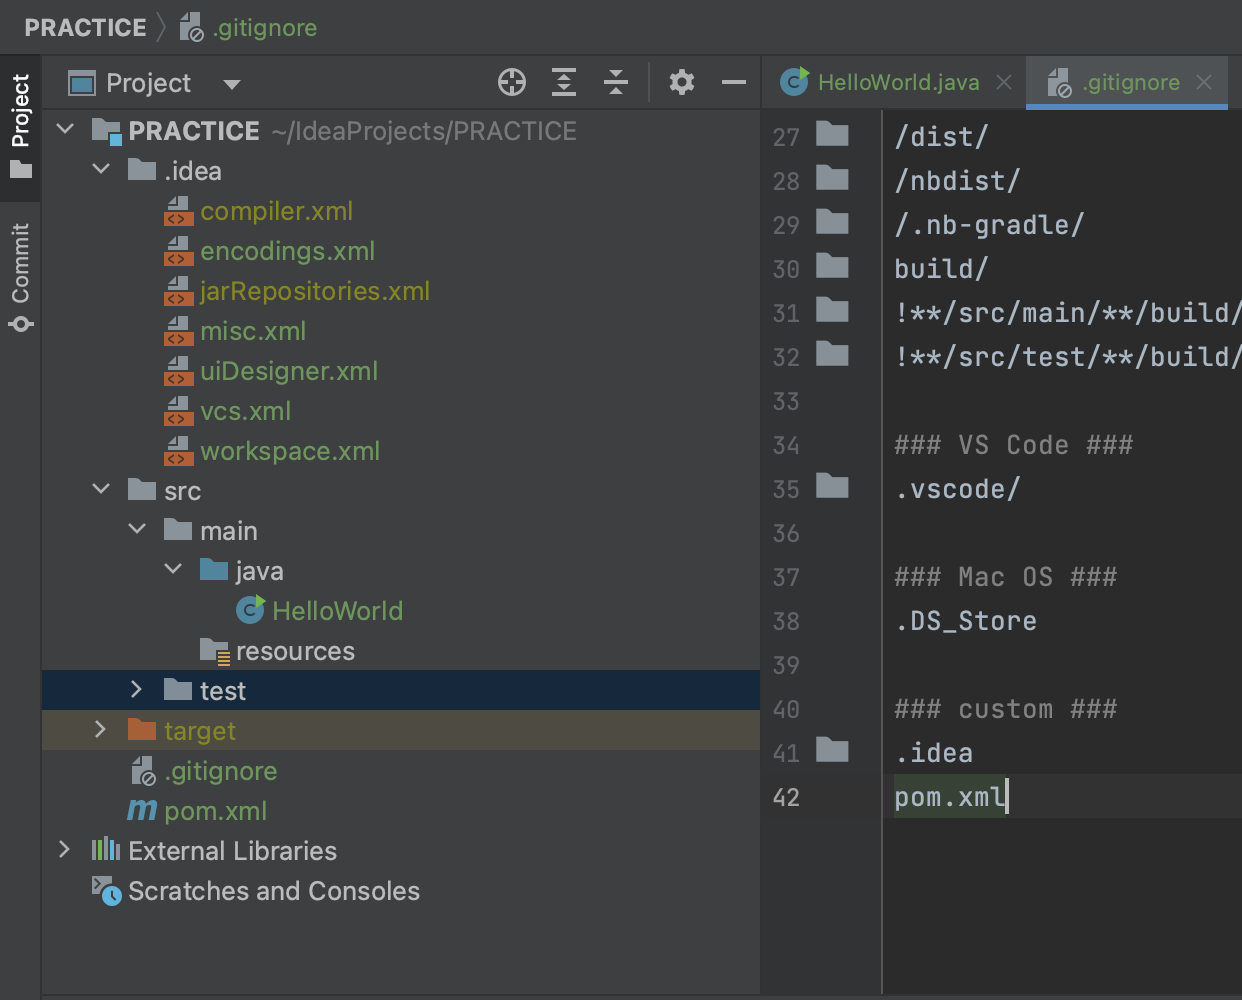
\includegraphics[width=0.75\linewidth]{src/gitignore.png}
        \caption{Обновленный .gitignore}
    \end{figure}
    
    Однако, как вы могли заметить, файл gitignore обновлен, 
    а некоторые файлы в папке \textit{.idea} и файл \textit{pom.xml} все еще отображаются как обновленные\\
    
    \textit{Ремарка: когда в Intellij IDEA или VSCode меняется файл gitignore, все изменения 
    (обновлен ли файл или может быть он untracked) видны в тот же момент}\\

    Это небольшая проблема, которую приходится чинить каждый раз, когда создается новый репозиторий в IDEA
    Достаточно прописать в терминале среды \texttt{git rm --cached -r -f .idea} и \texttt{git rm --cached -r -f pom.xml}

    \begin{figure}[H]
        \centering
        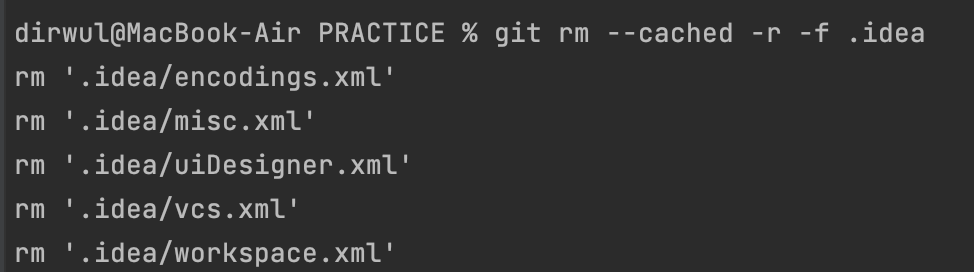
\includegraphics[width=0.75\linewidth]{src/cached.png}
        \caption{Изменение кэша локального гита}
    \end{figure}
    
    Таким образом, мы убрали папку и файл из кэша гита и теперь у нас все отображается (и работает) верно.

    \begin{figure}[H]
        \centering
        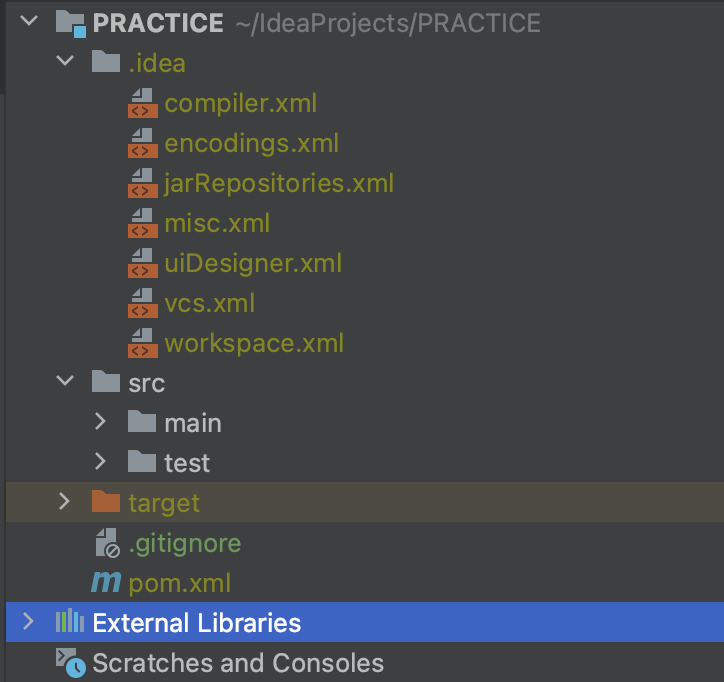
\includegraphics[width=0.75\linewidth]{src/untrack.png}
        \caption{Правильное состояние файлов}
    \end{figure}

    \newpage
    \section{Базовые операции с удаленным репозиторием}

    \subsection{New branch}

    Создаем новую ветку, которая наследуется от master и делаем в нее checkout (автоматически)

    \begin{figure}[H]
        \centering
        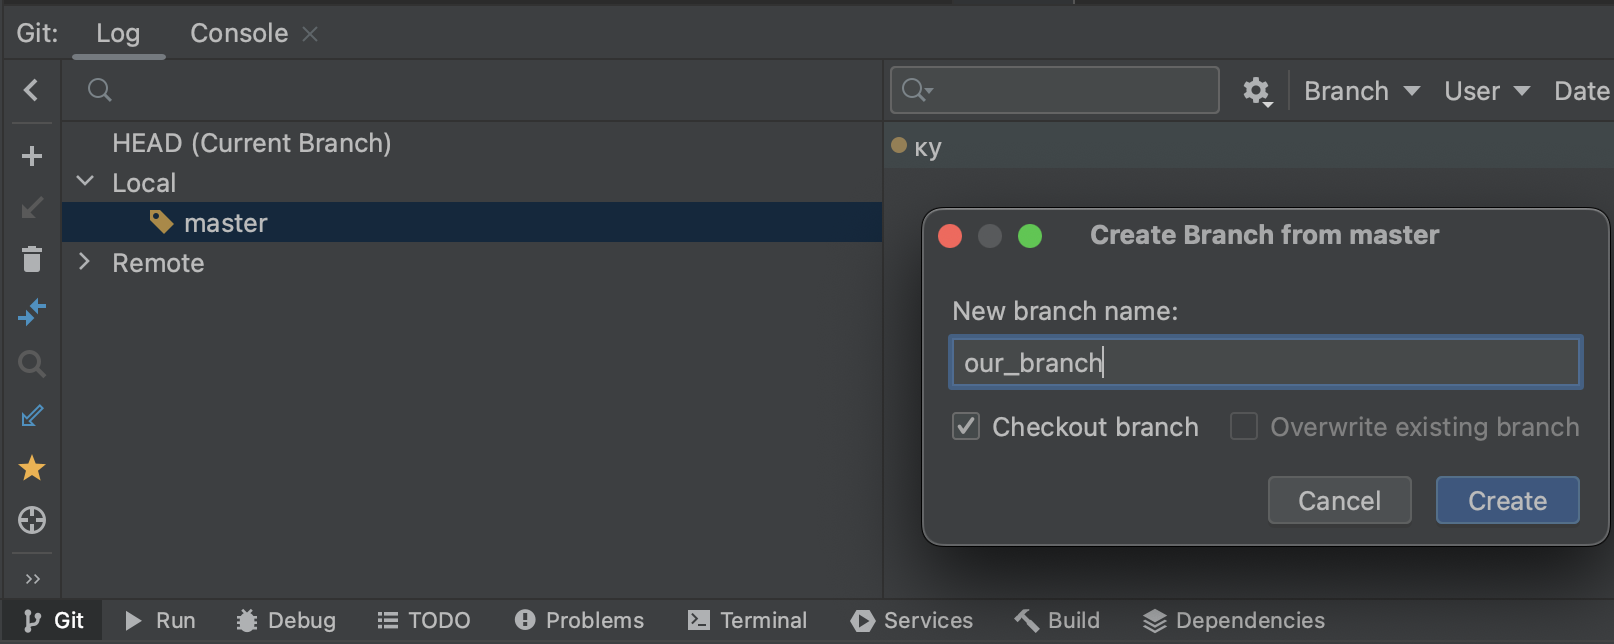
\includegraphics[width=0.75\linewidth]{src/newbranch.png}
        \caption{Новая ветка}
    \end{figure}

    \subsection{Commit}

    Хоткей: \textit{ctrl + K}
    Создаем коммит, указываем сообщение, прикрепленное к комиту и выбираем файлы, которые мы хотим
    внести в данный коммит

    \begin{figure}[H]
        \centering
        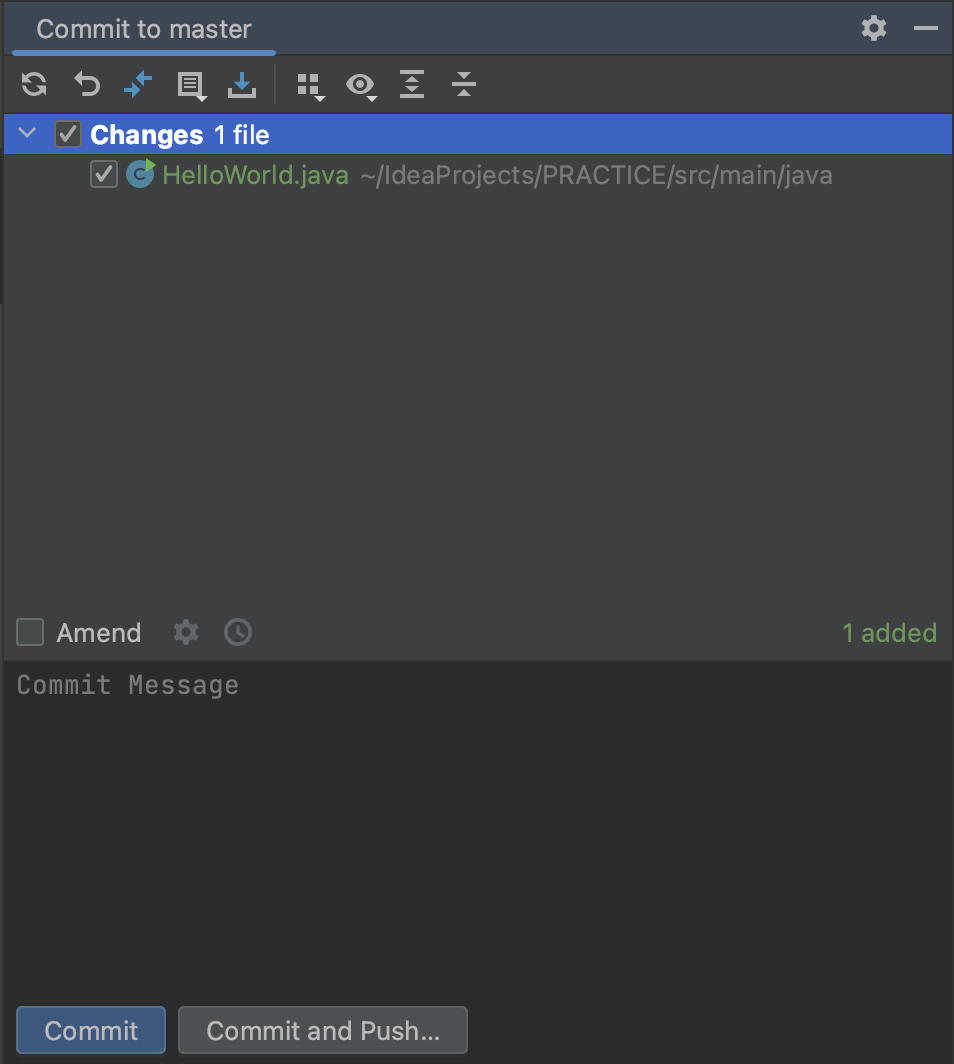
\includegraphics[width=0.55\linewidth]{src/commit.png}
        \caption{Коммит}
    \end{figure}

    \subsection{Push}

    Хоткей: \textit{shift + ctrl + K}
    Пушим уже имеющийся в локальном репозитории коммит

    \begin{figure}[H]
        \centering
        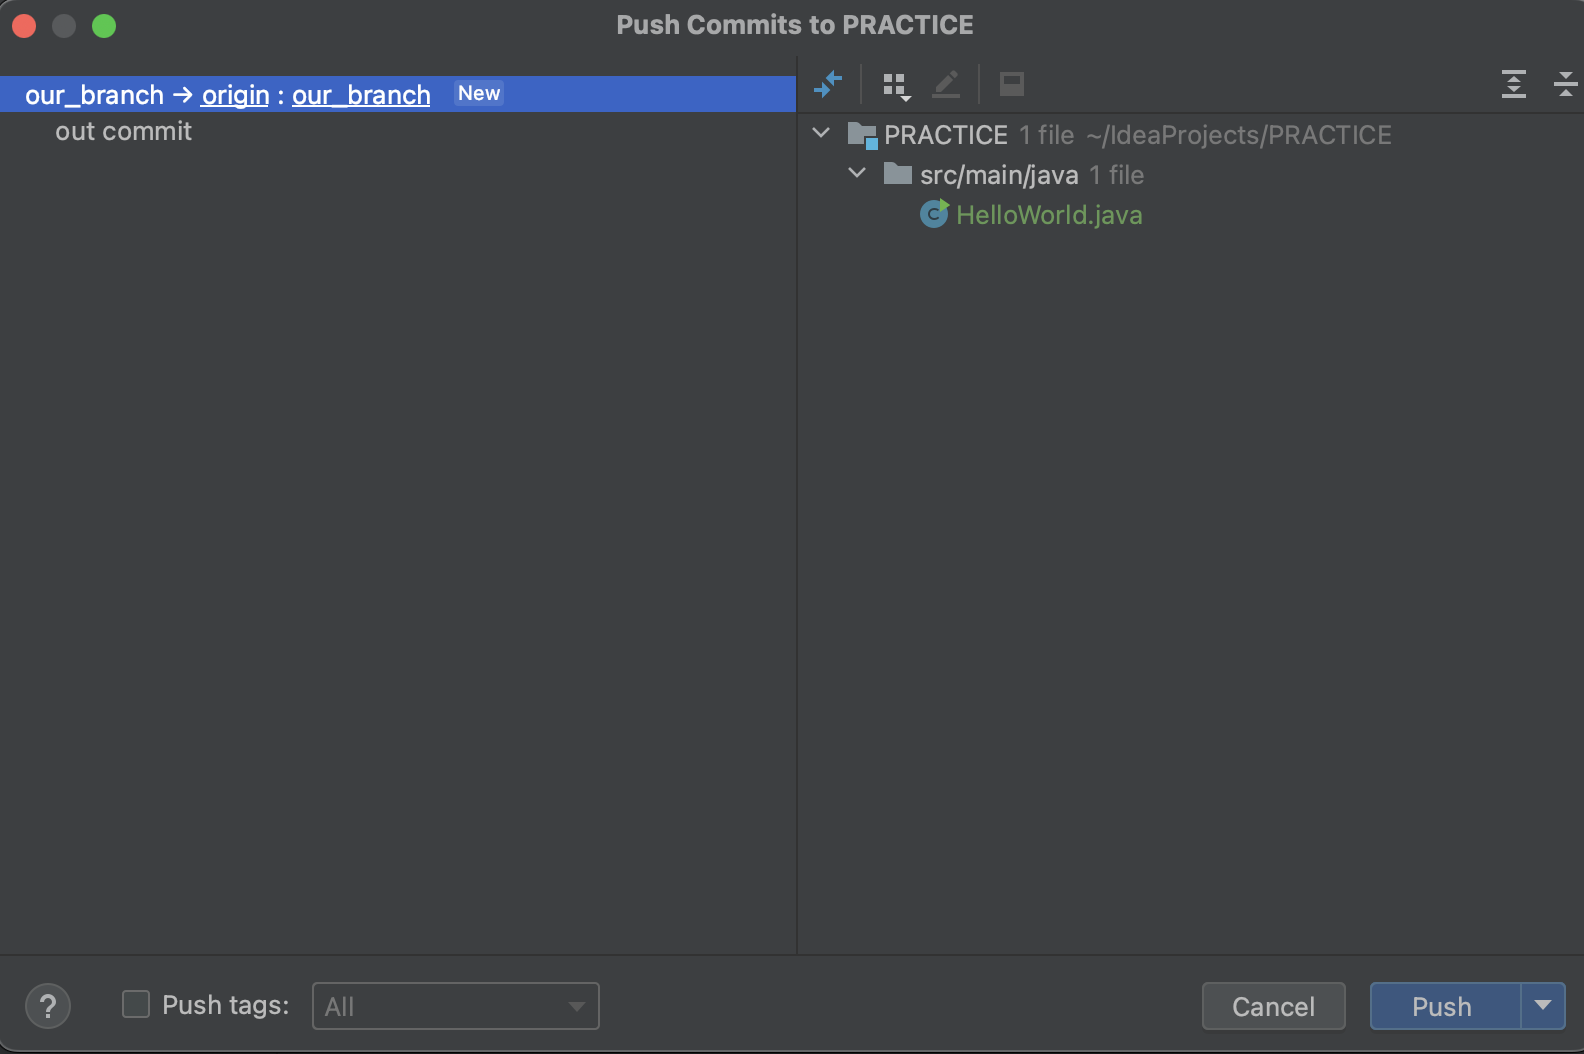
\includegraphics[width=0.75\linewidth]{src/push.png}
        \caption{Пуш}
    \end{figure}

    \subsection{Merge}

    Заходим в PR (PullRequest) панель слева и нажимаем \textit{command + N}
    Создаем наш PR и сразу же появится предложение сделать Merge.

    \begin{figure}[H]
        \centering
        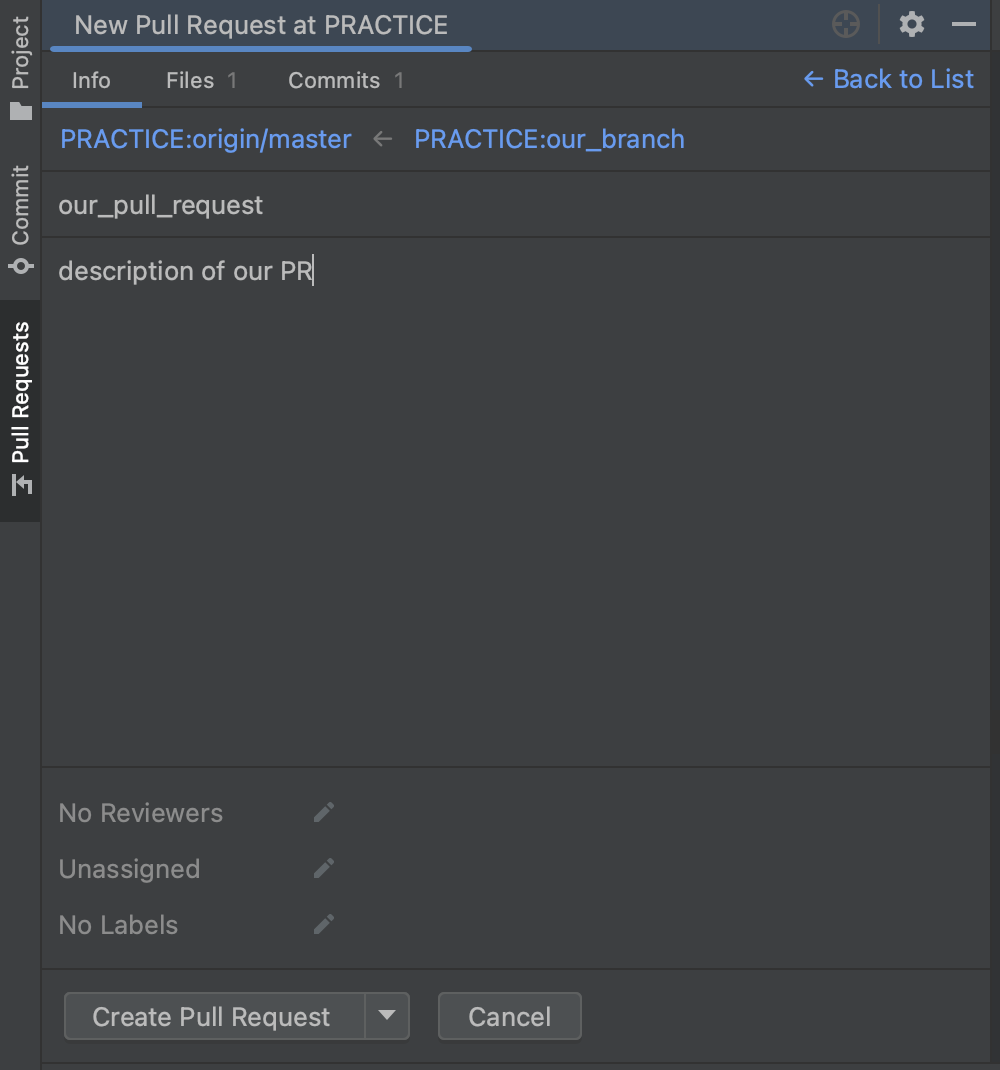
\includegraphics[width=0.55\linewidth]{src/PR.png}
        \caption{Pull Request}
    \end{figure}

    После чего делаем merge нашей ветки в master, если не требуется разрешить конфликт
    Если требуется - разрешаем конфликт и делаем merge
    
    \begin{figure}[H]
        \centering
        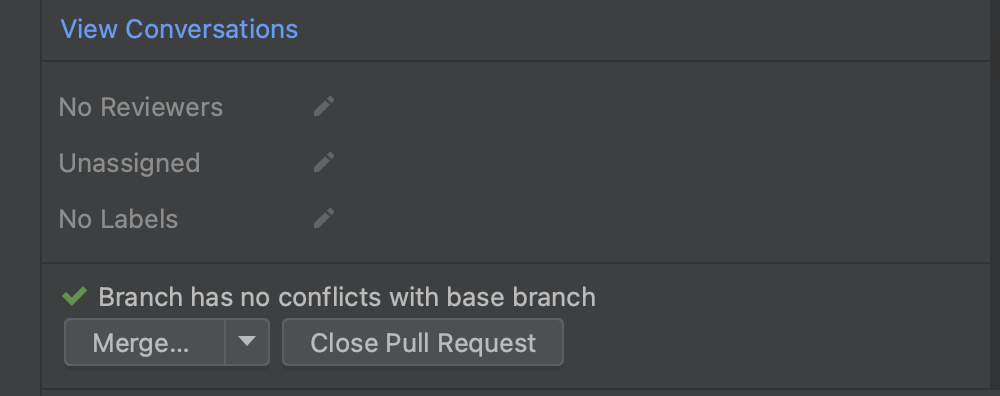
\includegraphics[width=0.75\linewidth]{src/merge.png}
        \caption{Merge}
    \end{figure}

    Далее мы переключаемся (checkout) на master ветку и нажимаем \textit{command + T}
    IDEA предлагает нам обновить нашу локальную master ветку

    \begin{figure}[H]
        \centering
        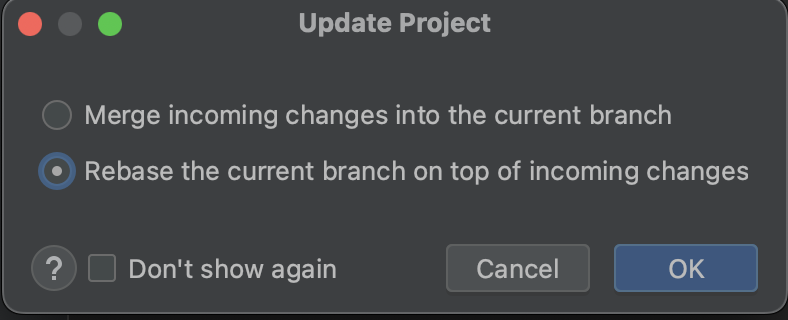
\includegraphics[width=0.75\linewidth]{src/rebase.png}
        \caption{Rebase}
    \end{figure}

    Делаем rebase и радуемся жизни!
    Все изменения так же видны в виде графа снизу:

    \begin{figure}[H]
        \centering
        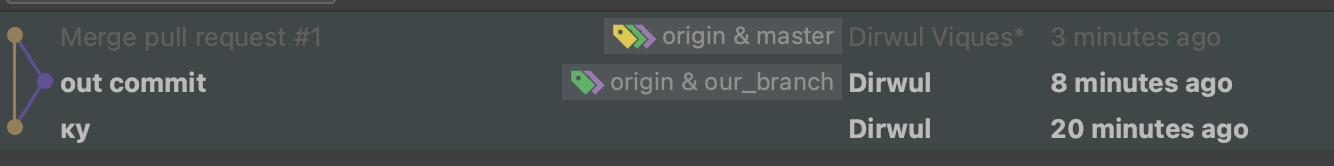
\includegraphics[width=0.75\linewidth]{src/gitactions.png}
        \caption{git actions}
    \end{figure}

\end{document}